\chapter{平面与空间直线}

\section{平面的方程}
\subsubsection*{平面的点法式方程}
\par 设在空间已经给定平面$\pi$,任取$\pi$上一个固定点$P(x_0,y_0,z_0)$,以及一个与$\pi$垂直的非零向量$\vb*{n}=(A,B,C)$,称$\vb*{n}$为平面的法线向量(简称为\textbf{法向量}),则平面$\pi$由点$P_0$和向量$\vb*{n}$惟一确定.
\par 设$P(x,y,z)$为平面上任一点,则方程
\begin{equation}\label{eq:pointnormalplane}
  A(x-x_0)+B(y-y_0)+C(z-z_0)=0
\end{equation}
可用来表示平面$\pi$,称为平面的点法式方程.

\subsubsection*{平面的一般式方程}
\par 将方程(\ref{eq:pointnormalplane})变形可得:
\begin{equation}
  Ax+By+Cz+D=0.
\end{equation}
\par 这一方程即为平面的一般式方程.
\par 利用平面的一般式方程,可以得到一系列在坐标系中有特殊位置的平面方程。譬如通过$x$轴的方程为$By+Cz=0$.请尝试推出通过原点、平行于坐标轴、通过坐标轴、垂直于坐标轴的特殊位置平面方程.

\subsubsection*{平面的截距式方程}
\par 设平面$\pi$在$x$,$y$,$z$轴上分别有截距$a$,$b$,$c$,其中$a$,$b$,$c$均为非0常数.设$P(x,y,z)$为平面上任一点,则方程
\begin{equation}
  \frac{x}{a}+\frac{y}{b}+\frac{z}{c}=1
\end{equation}
称为平面的截距式方程.

\subsubsection*{平面的参数式方程}
\par 设平面$\pi$过点$P(x_0,y_0,z_0)$,且有两个位于平面$\pi$上且不共线的向量$\vb*{a}=(L_1,M_1,N_1)$,$\vb*{b}=(L_2,M_2,N_2)$.设$P(x,y,z)$为平面上任一点,则
\begin{equation}\label{eq:paramplane}
  \begin{cases}
    x = x_0+sL_1+tL_2,                                         \\
    y = y_0+sM_1+tM_2, & (-\infty<s<+\infty,-\infty<t<+\infty) \\
    z = z_0+sN_1+tN_2.
  \end{cases}
\end{equation}
可用来表示平面$\pi$,称为平面的参数式方程.其中每一对$s$,$t$确定平面$\pi$上一点$P$.
\begin{example}
  已知平面的参数式方程,求平面的点法式方程?
  \begin{solution}
    根据方程\ref{eq:paramplane},立即可以写出平面过点$P(x_0,y_0,z_0)$,并写出平面内两个不共线的向量$\vb*{a}=(L_1,M_1,N_1)$,$\vb*{b}=(L_2,M_2,N_2)$.则可取法向量$\vb*{n}=\vb*{a} \times \vb*{b}$,即可写出点法式方程.
  \end{solution}
\end{example}

\section{空间直线的方程}
\subsubsection*{直线的参数式方程}
\par 设在空间已经给定直线$L$,任取$L$上一个固定点$P(x_0,y_0,z_0)$,以及一个与$L$平行的非零向量$\vb*{a}=(l,m,n)$,称$\vb*{a}$为直线$L$的\textbf{方向向量}.则方程
\begin{equation}\label{eq:paramline}
  \begin{cases}
    x = x_0+tl,                       \\
    y = y_0+tm, & (-\infty<t<+\infty) \\
    z = z_0+tn.
  \end{cases}
\end{equation}
可表示直线$L$,称为直线的参数式方程.若分别用$\vb*{r}$,$\vb*{r_0}$表示$P$,$P_0$的向径,则上式可写为
\begin{equation}
  \vb*{r}=\vb*{r_0}+t\vb*{a}.
\end{equation}
\subsubsection*{直线的对称式方程}
\par 将式\ref{eq:paramline}消去参数$t$,即可写成:
\begin{equation}\label{eq:symmetricline}
  \frac{x-x_0}{l}=\frac{y-y_0}{m}=\frac{z-z_0}{n}
\end{equation}
称为直线的对称式方程.对称式方程的几何意义也十分明显,它表示直线通过点$P(x_0,y_0,z_0)$,且以$\vb*{a}=(l,m,n)$为方向向量.
\begin{remark}
  值得注意的是,(\ref{eq:symmetricline})是比例式,这意味着$l$,$m$,$n$可能出现1或2个等于0的情形.
\end{remark}
\subsubsection*{直线的一般式方程}
\par 两平面相交得一直线.设两个不平行平面$\pi_1:a_1x+b_1y+c_1z+d_1=0$,$\pi_2:a_2x+b_2y+c_2z+d_2=0$,则交线可由两平面方程联立所得的方程组来表示。即
\begin{equation}\label{eq:normalline}
  \begin{cases}
    a_1x+b_1y+c_1z+d_1=0, \\
    a_2x+b_2y+c_2z+d_2=0. \\
  \end{cases}
\end{equation}
\begin{example}
  已知直线的一般式方程,求直线的参数式方程或对称式方程?
  \begin{solution}
    由方程组\ref{eq:normalline},并根据几何性质,立即可以写出直线的方向向量$\vb*{a}=(a_1,b_1,c_1) \times (a_2,b_2,c_2)$.又因为方程组\ref{eq:normalline}一定有非零解(第4章将说明这个问题),可以求得直线上一点.则参数式或对称式方程可以写出.
  \end{solution}
\end{example}

\section{两个平面的位置关系}
\begin{definition}[两个平面的夹角]
  设两个平面$\pi_1$,$\pi_2$的两个法向量分别为$\vb*{n_1}$,$\vb*{n_2}$,则我们把这两个法向量的夹角$\theta$称为这两个平面的夹角(通常取锐角,与高中阶段的二面角不同).$\theta$可由
  \begin{equation*}
    \cos{\theta} =  \frac{|\vb*{n_1} \cdot \vb*{n_2}|}{\| \vb*{n_1} \|\| \vb*{n_2} \|}
  \end{equation*}
  来确定.
\end{definition}
\par 特别的,有
\begin{enumerate}
  \item $\pi_1$与$\pi_2$平行 $\Leftrightarrow$ $\vb*{n_1} \parallel \vb*{n_2}$
  \item $\pi_1$与$\pi_2$垂直 $\Leftrightarrow$ $\vb*{n_1} \perp \vb*{n_2}$
\end{enumerate}
\par 对于平面$\pi_1:a_1x+b_1y+c_1z+d_1=0$,$\pi_2:a_2x+b_2y+c_2z+d_2=0$,从几何上看,它们的位置关系只有3种可能,即\textbf{相交}、\textbf{平行而不重合}以及\textbf{重合};从代数上看,总结如下:
\begin{enumerate}
  \item $\pi_1$与$\pi_2$相交 $\Leftrightarrow$ $\vb*{n_1}$与$\vb*{n_2}$不平行 $\Leftrightarrow$ $a_1:b_1:c_1 \not= a_2:b_2:c_2$
  \item $\pi_1$与$\pi_2$平行而不重合 $\Leftrightarrow$ $\frac{a_1}{a_2}=\frac{b_1}{b_2}=\frac{c_1}{c_2} \not= \frac{d_1}{d_2}$
  \item $\pi_1$与$\pi_2$重合 $\Leftrightarrow$ $\frac{a_1}{a_2}=\frac{b_1}{b_2}=\frac{c_1}{c_2} = \frac{d_1}{d_2}$
\end{enumerate}
\begin{remark}
我们一般认为,重合是一种特殊的平行.
\end{remark}
\begin{example}
  求通过点$P_1(-1,0,2)$,$P_2(1,1,1)$,且与平面$x+y+z+1=0$垂直的平面的方程.
  \begin{solution}
    设所求平面的法向量为$\vb*{n}$,则由几何关系易知$\vb*{n} \perp \overrightarrow{P_1P_2} $,$\vb*{n} \perp (1,1,1)$,于是可取
    \begin{equation*}
      \vb*{n} = \overrightarrow{P_1P_2} \times (1,1,1) = (2,-3,1)
    \end{equation*}
    再任意使用$P_1$或$P_2$作为点法式中的“点”,可求得平面的点法式方程,化简为$2x-3y+z=0$.
  \end{solution}
  \begin{remark}
    在高中阶段,我们可能更习惯于将$\vb*{n}$的三个坐标设出,利用两个垂直条件联立求非零解.这个题目提供给了我们一种求法向量的新思路,也即使用叉乘.
    \par 另外,若题目没有要求,为了减少失误,通常我们求平面方程写到点法式即可,不需要转化为一般式.
  \end{remark}
\end{example}


\section{两条直线的位置关系}
\begin{definition}[两条直线的夹角]
  设两个平面$L_1$,$L_2$的两个方向向量分别为$\vb*{a_1}$,$\vb*{a_2}$,则我们把这两个方向向量的夹角$\theta$称为这两条直线的夹角(通常取锐角).$\theta$可由
  \begin{equation*}
    \cos{\theta} =  \frac{|\vb*{a_1} \cdot \vb*{a_2}|}{\| \vb*{a_1} \|\| \vb*{a_2} \|}
  \end{equation*}
  来确定.
\end{definition}
\par 特别的,有
\begin{enumerate}
  \item $L_1$与$L_2$平行 $\Leftrightarrow$ $\vb*{a_1} \parallel \vb*{a_2}$
  \item $L_1$与$L_2$垂直 $\Leftrightarrow$ $\vb*{a_1} \perp \vb*{a_2}$
\end{enumerate}
% \par 对于直线$L_1:\frac{x-x_1}{l_1}+\frac{y-y_1}{m_1}+\frac{z-z_1}{n_1}$,$L_2:\frac{x-x_2}{l_2}+\frac{y-y_2}{m_2}+\frac{z-z_2}{n_2}$,从几何上看,它们的位置关系只有4种可能,即异面、相交于一点、平行而不重合或重合;从代数上看,取$L_1$上一点$P_1$,$L_2$上一点$P_2$总结如下:
\par 对于上述两条直线,从几何上看,它们的位置关系只有4种可能,即\textbf{异面}、\textbf{相交于一点}、\textbf{平行而不重合}或\textbf{重合};从代数上看,取$L_1$上一点$P_1$,$L_2$上一点$P_2$,总结如下:
\begin{enumerate}
  % \not \parallel 有问题
  \item $L_1$与$L_2$异面 $\Leftrightarrow$ 三个向量$\vb*{a_1}$,$\vb*{a_2}$,$\overrightarrow{P_1P_2}$不共面
  \item $L_1$与$L_2$相交于一点 $\Leftrightarrow$ 三个向量$\vb*{a_1}$,$\vb*{a_2}$,$\overrightarrow{P_1P_2}$共面且$\vb*{a_1} \not\parallel \vb*{a_2}$
  \item $L_1$与$L_2$平行而不重合 $\Leftrightarrow$ $\vb*{a_1} \parallel \vb*{a_2} \not\parallel \overrightarrow{P_1P_2}$
  \item $L_1$与$L_2$重合 $\Leftrightarrow$ $\vb*{a_1} \parallel \vb*{a_2} \parallel \overrightarrow{P_1P_2}$
\end{enumerate}
\par 另外,$L_1$与$L_2$共面 $\Leftrightarrow$ 三个向量$\vb*{a_1}$,$\vb*{a_2}$,$\overrightarrow{P_1P_2}$共面 $\Leftrightarrow$ $[\vb*{a_1} \quad \vb*{a_2} \quad \overrightarrow{P_1P_2}]=0$
\begin{remark}
  判断两直线共面,有两种方法,一是使用上述混合积的方法;二是先判断是否平行(平行一定共面,用方向向量判断),若不平行,判断是否相交(联立直线方程观察有无解).
\end{remark}

\section{直线与平面的位置关系}
\begin{definition}[直线与平面的夹角]
  \par 一条直线$L$与$L$在平面$\pi$上的投影直线的夹角$\varphi$, 称为直线$L$与平面$\pi$的夹角.
  \par 当$L$与$\pi$垂直时,规定$L$与$\pi$的夹角为$\frac{\pi}{2}$.
\end{definition}
\par 设$\vb*{a}$是直线$L$的方向向量, $\vb*{n}$是平面$\pi$的法向量.特别的,有
\begin{enumerate}
  \item $L$与$\pi$平行 $\Leftrightarrow$ $\vb*{a} \perp \vb*{n}$
  \item $L$与$\pi$垂直 $\Leftrightarrow$ $\vb*{a} \parallel \vb*{n}$
\end{enumerate}
\par 对于平面$\pi:Ax+By+Cz+D=0$和直线$L:\frac{x-x_0}{l}=\frac{y-y_0}{m}=\frac{z-z_0}{n}$,对二者交点的讨论如下:
\begin{enumerate}
  \item 当$Al+Bm+Cn \not= 0$时,$L$与$\pi$交于一点
  \item 当$Al+Bm+Cn = 0$时,若$Ax_0+By_0+Cz_0+D \not= 0$,则$L$与$\pi$平行
  \item 当$Al+Bm+Cn = 0$时,若$Ax_0+By_0+Cz_0+D = 0$,则$L$在平面$\pi$上
\end{enumerate}
\begin{remark}
  以上三个小节关于位置关系的问题,本质上都可以通过将方程联立,讨论解的个数,从而将其代数化.请尝试用这一思想证明上述关于直线与平面交点的讨论.
\end{remark}

\section{距离}
\subsubsection*{点到平面的距离}
\par 给定平面$\pi:Ax+By+Cz+D=0$以及平面$\pi$外一点$P_1(x_1,y_1,z_1)$,取平面$\pi$上一点$P_0(x_0,y_0,z_0)$.则点$P_1$到平面$\pi$的距离$d$为
\begin{equation}
  d=\frac{|Ax_1+By_1+Cz_1+D|}{\sqrt{A^2+B^2+C^2}}
\end{equation}
称为\textbf{点到平面的距离公式}.
\begin{remark}
  注意到$d$为$\overrightarrow{P_0 P_1}$在平面 的法向量$\vb*{n}$上射影的绝对值,请尝试推导点到平面的距离公式.另外,这个公式在形式上与二维平面内点到直线的距离公式非常类似,可以联系记忆.
\end{remark}
\subsubsection*{点到直线的距离}
\par 给定直线$L$以及直线$L$外一点$P_1(x_1,y_1,z_1)$,取直线$L$上一点$P_0(x_0,y_0,z_0)$,直线$L$的方向向量为$\vb*{a}$.则点$P_1$到直线$L$的距离$d$为
\begin{equation}
  d=\frac{\|\overrightarrow{P_0 P_1} \times \vb*{a}\|}{\|\vb*{a}\|}
\end{equation}
称为\textbf{点到直线的距离公式}.
\begin{remark}
  这一公式的推导和记忆都可以借助几何方法.$\|\overrightarrow{P_0 P_1} \times \vb*{a}\|$表示平行四边形的面积,除以底边长度$\|\vb*{a}\|$即为高.如图 \ref{fig:pointlinedistance}.
\end{remark}

\begin{marginfigure}[7em]
	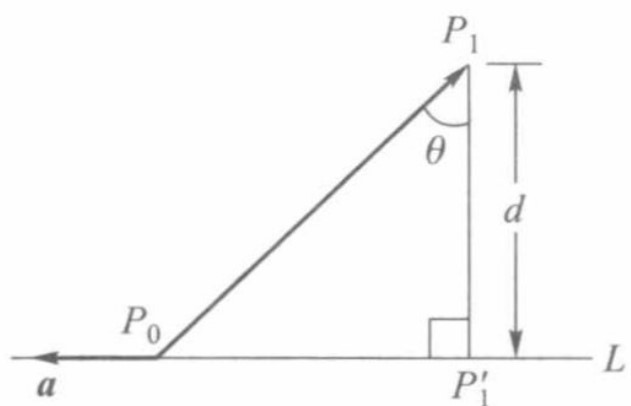
\includegraphics[width=\marginparwidth]{figures/point-line-distance.jpg}
	\caption{点到直线的距离}
	\label{fig:pointlinedistance}
\end{marginfigure}

\subsubsection*{异面直线的距离}
\par 所谓异面直线$L_1$与$L_2$的距离,是指两直线上的点之间的最短距离.设直线$L_1$,$L_2$的方向向量分别为$\vb*{a_1}$,$\vb*{a_2}$,取直线$L_1$上一点$P_1$,$L_2$上一点$P_2$.则两直线的距离$d$为
\begin{equation}
  d=\frac{|[\vb*{a_1} \quad \vb*{a_2} \quad \overrightarrow{P_1P_2}]|}{\|\vb*{a_1} \times \vb*{a_2}\|}
\end{equation}
称为\textbf{点到直线的距离公式}.
\begin{remark}
  这一公式的推导和记忆都可以借助几何方法.$|[\vb*{a_1} \quad \vb*{a_2} \quad \overrightarrow{P_1P_2}]|$表示以$\vb*{a_1}$,$\vb*{a_2}$为邻边构成的平行四边形为底,以$\overrightarrow{P_1P_2}$为侧棱的平行六面体的体积,除以底面积$\|\vb*{a_1} \times \vb*{a_2}\|$,即为高.
\end{remark}